
\documentclass[letterpaper,11pt]{article}

\usepackage{latexsym}
\usepackage{amsmath}
\usepackage{amssymb}
\usepackage{fancyhdr}
\usepackage[margin=1.0in, left=0.5in, right=0.5in, top=1.25in, headsep=10mm, headheight=15mm]{geometry}
\usepackage{graphicx}

\pagestyle{fancy}
\rhead{Michael Deakin\\Math 516\\Homework 2}

\newcommand*\limitset[1]{{#1}^\prime}
\newcommand*\closure[1]{\overline{#1}}
\newcommand*\closureunion[1]{{#1}\cup \limitset{#1}}
\newcommand*\interior[1]{{#1}^\circ}
% The set of points within some distance #1 from #2
\newcommand*\neighbor[2]{N_{#1}({#2})}
% The neighborhood without #2
\newcommand*\delneighbor[2]{N_{#1}^*({#2})}
\newcommand*\set[1]{\{ #1 \} }
\newcommand*\conjugate[1]{\overline{#1}}
\newcommand*\sequence[2]{\set{#1}_{#2=1}^\infty}
\newcommand*\series[2]{\sum_{#2=1}^\infty #1_{#2}}
\newcommand*\compose[2]{#1 \circ #2}
\newcommand*\udisk[0]{\mathbb{D}}
\newcommand*\disk[2]{D_{#1}(#2)}
\newcommand*\punctdisk[2]{\disk_{ #1 } - \set{#2}}
\newcommand*\complex[0]{\mathbb{C}}
\newcommand*\naturals[0]{\mathbb{N}}
\newcommand*\rationals[0]{\mathbb{Q}}
\newcommand*\reals[0]{\mathbb{R}}

\newcommand*\domain[0]{\Omega}
\newcommand*\bndry[1]{\partial #1}
\newcommand*\bndrydom[0]{\partial \domain}
\newcommand*\compactcont[0]{\subset \subset} % U \compactcont V \rightarrow U \subset \closure{U} \subset V, where U, V are (open) domains

\newcommand*\ball[2]{B_{#2}(#1)}

\newcommand*\limitto[2]{\lim \limits_{#1 \rightarrow #2}}

\newcommand{\dd}[1]{\;\mathrm{d}#1}
\newcommand{\dx}{\dd{x}}
\newcommand{\dy}{\dd{y}}
\newcommand{\dz}{\dd{z}}
\newcommand{\ds}{\dd{s}}
\newcommand{\dt}{\dd{t}}
\newcommand*\pderiv[2]{\frac{\partial #1}{\partial #2}}
\newcommand*\nthpderiv[3]{\frac{\partial^{#3} #1}{\partial #2^{#3}}}
\newcommand*\deriv[2]{\frac{\dd{#1}}{\dd{#2}}}
\newcommand*\nthderiv[3]{\frac{\dd{^{#3} #1}}{\dd{#2^{#3}}}}

\DeclareMathOperator{\res}{res}
\DeclareMathOperator{\sign}{sign}
\DeclareMathOperator{\diam}{diam}
\DeclareMathOperator{\partition}{Partition}

% Average integral from https://tex.stackexchange.com/questions/759/average-integral-symbol
\def\Xint#1{\mathchoice
{\XXint\displaystyle\textstyle{#1}}%
{\XXint\textstyle\scriptstyle{#1}}%
{\XXint\scriptstyle\scriptscriptstyle{#1}}%
{\XXint\scriptscriptstyle\scriptscriptstyle{#1}}%
\!\int}
\def\XXint#1#2#3{{\setbox0=\hbox{$#1{#2#3}{\int}$ }
\vcenter{\hbox{$#2#3$ }}\kern-.6\wd0}}
\def\ddashint{\Xint=}
\def\dashint{\Xint-}
\def\avgint{\dashint}

\begin{document}

I collaborated with Damien Huet on this assignment

\begin{enumerate}
\item \begin{enumerate}
\item
  Let $\xi \in \bndrydom$ and $w(x)$ be a barrier on $\domain_1 \compactcont \domain$ with $w$ superharmonic in $\domain_1$, $w > 0$
  in $\closure{\domain}_1 \setminus \set{\xi}$, $w(\xi) = 0$.
  Show that $w$ can be extended to a barrier in $\domain$.

  Let's rewrite this to what I think is meant by the problem:
  First, $\xi \in \bndrydom$, but $\xi \notin \bndrydom_1$, since $\closure{\domain}_1 \subset \domain$.
  Next, $w$ is superharmonic on $\domain_1$, and $w > 0$ on $\bndrydom_1$.
  Then we want to show that we can construct an extension $\tilde{w}$ of $w$ from $\domain_1$ s.t.
  $\tilde{w}(\xi) = 0$, $\tilde{w} > 0$ on $\bndrydom$, and $\tilde{w}$ is superharmonic on $\domain$.

  Let $m = \inf \limits_{\domain_1} w$ and
  $$
  w_0(x) =
  \begin{cases}
    \min(m, w(x)) & x \in \closure{\domain}_1\\
    m & x \in \domain \setminus \closure{\domain}_1
  \end{cases}
  $$

\item
  Let $\domain = \set{x^2 + y^2 < 1} \setminus \set{-1 \leq x \leq 0, y = 0}$.
  Show that the function $w := -Re\left( \frac{1}{\ln(z)} \right) = - \frac{\log(r)}{(\log(r))^2 + \theta^2}$ is a local barrier at $\xi = 0$.

  First we need to show that there is a neighborhood $N$ s.t.
  for all $B \compactcont N$ and all harmonic $h$ in $B$ with $h(x) \leq w(x)$ for $x \in \bndry{B}$,
  we have $w \geq h$ for $x \in B$.

  This can be shown with complex analysis.
  First note that since $\domain$ is simply connected and excludes $0$, the logarithm exists on it, and is holomorphic.
  Next define $W(z) = \frac{1}{\ln(z)}$.
  $W$ is a composition of holomorphic functions on $\domain$, and thus, its real and imaginary parts are harmonic.
  Note that $w(x, y) = Re(W(x + i y))$ shows that $w$ is harmonic on $\domain$.
  From the notes on superharmonic functions, we know that harmonic functions are always superharmonic functions.
  Therefore, we can take any neighborhood $N \compactcont \domain$ we want and $w$ will be superharmonic on it.

  Next we need to show that in the closure of such a neighborhood, $w(x, y) > 0$ when $x^2 + y^2 \neq 0$.

  Since $0 < r^2 = x^2 + y^2 < 1$, $\log \left( r \right) < 0$.
  Then since $(\log(r))^2 + \theta^2 > 0$, $-\frac{\log(r)}{(log(r))^2 + \theta^2} > 0$.
  Since this is true for $\domain$, it's true for $N$ as well.

  Finally we note that $0 \leq \lim \limits_{r \rightarrow 0+} \left| \frac{\ln(r)}{(\ln(r))^2 + \theta^2} \right| \leq \lim \limits_{r \rightarrow 0+} \frac{1}{|\ln(r)|} = 0$,
  so we must have $w(0) = 0$ for this to be continuous.

  Thus, $w$ is a local barrier for $\xi = 0$ in $\domain$.
\end{enumerate}

\item \begin{enumerate}
\item
  Show that the problem of minimizing energy
  $$
  I[u] = \int_J x^2 |u'(x)|^2 \dx
  $$
  for $u \in C(\closure{J})$ with piecewise continuous derivatives in $J := (-1, 1)$,
  satisfying the boundary conditions $u(-1) = 0$, $u(1) = 1$ is not attained.

  Consider
  $$
  u_k(x) =
  \begin{cases}
    0 & -1 \leq x \leq -\frac{1}{k}\\
    \frac{k^2}{2} x^2 + k x + \frac{1}{2} & -\frac{1}{k} \leq x \leq 0\\
    -\frac{k^2}{2} x^2 + k x + \frac{1}{2} & 0 \leq x \leq \frac{1}{k}\\
    1 & \frac{1}{k} \leq x \leq 1\\
  \end{cases}
  $$

  $u_k$ has piecewise continuous derivatives, is $0$ at $-1$ and $1$ at $1$.
  Furthermore, $I[u_k] \leq \frac{C}{k}$ for some positive $C$ indepenedent of $k$,
  and thus, $\lim \limits_{k \rightarrow \infty} I[u_k] = 0$ is our minimal energy.
  However, $\lim \limits_{k \rightarrow \infty} u_k$ does not have piecewise continuous derivatives though, so it's not in the admissible set.
  Thus, $\inf_{u} I[u] = 0$, and now we must show it's not actually attainable.

  By the intermediate value theorem, since $u(-1) = 0$ and $u(1) = 1$, there is some $y \in (-1, 1)$ s.t. $u'(y) = \frac{1}{2}$.
  Then since $u'(x)$ is piecewise continuous, we can choose some $\delta > 0$ s.t. $0 < \epsilon < u'(x)$ whenever $|x - y| < \delta$.
  Then $\int \limits_{-1}^{1} x^2 u'(x)^2 \dx \geq \int \limits_{y - \delta}^{y + \delta} x^2 \epsilon^2 \dx > 0$.
  Thus, since the optimal energy is $0$, and any element in the admissible set has non-zero energy, the minimizer is not attained.

\item
  Consider the problem of minimizing the energy
  $$
  I[u] = \int_0^1 (1 + |u'(x)|^2)^{\frac{1}{4}} \dx
  $$
  for all $u \in C^1((0, 1)) \cap C([0, 1])$ satisfying $u(0) = 0, u(1) = 1$. Show that the minimum is $1$ and is not attained.

  Consider
  $$
  u_k(x) =
  \begin{cases}
    -k^2 x^2 + 2 k x & 0 \leq x \leq \frac{1}{k}\\
    1 & \frac{1}{k} \leq x \leq 1\\
  \end{cases}
  $$

  $u_k$ has piecewise continuous derivatives, is $0$ at $0$ and $1$ at $1$.
  Furthermore, $I[u_k] \leq \frac{k - 1}{k} + \frac{(1 + 4 k^2)^{1/4}}{k}$,
  and thus, $\lim \limits_{k \rightarrow \infty} I[u_k] = 1$ is our minimal energy.
  However, $\lim \limits_{k \rightarrow \infty} u_k$ does not have piecewise continuous derivatives though, so it's not in the admissible set.
  Thus, $\inf_{u} I[u] = 1$, and now we must show it's not actually attainable; this is largely the same process as in 2a.

  By the intermediate value theorem, since $u(0) = 0$ and $u(1) = 1$, there is some $y \in (0, 1)$ s.t. $u'(y) = 1$.
  Then since $u'(x)$ is piecewise continuous, we can choose some $\delta > 0$ s.t. $0 < \epsilon < u'(x)$ whenever $|x - y| < \delta$.
  Then
  $$
  \int \limits_{0}^{1} (1 + u'(x)^2)^{1/4} \dx \geq \int \limits_{y - \delta}^{y + \delta} (1 + \epsilon^2)^{1/4} \dx + 1 - 2 \delta
  = 1 - 2 \delta + 2 \delta (1 + \epsilon^2)^{1/4} > 1
  $$
  Thus, since the optimal energy is $1$, and any element in the admissible set has energy greater than 1, the minimizer is not attained.
\end{enumerate}

\item Discuss the Dirichlet Principle for
$$
\begin{cases}
  \Delta^2 u(x) = f(x) & x \in \domain\\
  u(x) = \pderiv{u}{\nu}(x) = 0 & x \in \bndrydom
\end{cases}
$$

\item Let
$$
\Phi(x - y, t) = (4 \pi t)^{-n / 2} e^{-\frac{|x - y|^2}{4t}}
$$
\begin{enumerate}
\item Show that there exists a generic constant $C_n$ s.t.
  $$
  \Phi(x - y, t) \leq C_n |x - y|^{-n}
  $$
  (Hint: Maximize the function in $t$)

  Following the hint, we compute

  $$
  0 = \deriv{\Phi(r, t)}{t}
    = - \frac{n}{2} (4 \pi t)^{-\frac{n}{2} - 1} 4 \pi e^{-\frac{r^2}{4 t}} + (4 \pi t)^{-n / 2} e^{-\frac{r^2}{4 t}} \left( \frac{r^2}{4 t^2} \right)
  $$

  Then, after some simplification we get

  $$
  \frac{n}{2} (4 \pi t)^{-\frac{n}{2} - 1} 4 \pi = (4 \pi t)^{-n / 2} \left( \frac{r^2}{4 t^2} \right)
  $$

  which leaves us with just

  $$
  t_{crit} = \frac{r^2}{2 n}
  $$

  Then for this to be a local maximum, we need $\nthderiv{\Phi}{t}{2}(r, t_{crit}) < 0$.
  After some computation, we arrive at

  $$
  \nthderiv{\Phi}{t}{2}(r, t_{crit}) = -\frac{2 n^3 \left( \frac{2 \pi r}{n} \right)^{-n / 2} e^{-n / 2}}{r^4} < 0
  $$

  Thus, this is a local maximum. Then

  $$
  \Phi(r, t) \leq \Phi(r, t_{crit}) = \left( r \sqrt{\frac{2 \pi}{n}} \right)^{-n} e^{-n / 2} \leq C r^{-n}
  $$

  for some $C$ independent of $R$.

\item
  Let $n = 1$ and $f(x)$ be a bounded measurable function s.t. $f(x_0 -)$ and $f(x_0+)$ exists.
  Show that
  $$
  \limitto{t}{0} \int_R \Phi(x_0  - y, t) f(y) \dy = \frac{1}{2} (f(x_0-) + f(x_0+))
  $$

  $f$ is bounded and measurable.
  This is essentially a generalization of the proof for Theorem 2.3.1 in the book.

  First define $u(x, t) = \int_\reals \Phi(x_0 - y, t) f(y) \dy$.
  Then consider $u(x, t) - \frac{1}{2} f(x_0+) - \frac{1}{2} f(x_0-)$
  Since $f(x_0-)$ and $f(x_0+)$ exists, given any $\epsilon > 0$, we can choose $\delta > 0$ s.t.
  for $|y - x_0| < \delta$, we have

  $$
  \begin{cases}
    |f(y) - f(x_0+)| < \epsilon & y < x_0\\
    |f(y) - f(x_0-)| < \epsilon & y > x_0\\
  \end{cases}
  $$

  Now we write

  \begin{align*}
  u(x_0, t) & - \frac{1}{2} f(x_0+) - \frac{1}{2} f(x_0-)\\
    = & \int_\reals \Phi(x_0 - y, t) \left[  f(y) - \frac{1}{2} f(x_0+) - \frac{1}{2} f(x_0-) \right] \dy\\
    = & \int_{B_\delta(x_0)} \Phi(x_0 - y, t) \left[  f(y) - \frac{1}{2} f(x_0+) - \frac{1}{2} f(x_0-) \right] \dy\\
      & + \int_{B_\delta(x_0)^c} \Phi(x_0 - y, t) \left[  f(y) - \frac{1}{2} f(x_0+) - \frac{1}{2} f(x_0-) \right] \dy\\
    = & I_t + J_t
  \end{align*}

  $\limitto{t}{0} J_t = 0$ as shown in the book,
  as $f(y) - \frac{1}{2} f(x_0+) - \frac{1}{2} f(x_0+) < C$ since $f$ is bounded,
  letting us bound
  $|J_t| < \frac{C}{\sqrt{t}} \int_{\ball{x_0}{\delta}^c} e^{-\frac{|x_0 - y|^2}{4 t}} \dy \leq C \int_{\ball{x_0}{(\delta / \sqrt{t})}^c} e^{-\frac{|\tilde{x}_0 - \tilde{y}|^2}{16}} \dd{\tilde{y}}$

  Thus we only need to concern ourselves with $\limitto{t}{0} I_t$.

  \begin{align*}
  I_t = &\int_{B_\delta(x_0)} \Phi(x_0 - y, t) \left[ f(y) - \frac{1}{2} f(x_0+) - \frac{1}{2} f(x_0-) \right] \dy\\
      = &\int \limits_{x_0 - \delta}^{x_0} \Phi(x_0 - y, t) \left[ f(y) - \frac{1}{2} f(x_0+) - \frac{1}{2} f(x_0-) \right] \dy\\
        &+ \int \limits_{x_0}^{x_0 + \delta} \Phi(x_0 - y, t) \left[ f(y) - \frac{1}{2} f(x_0+) - \frac{1}{2} f(x_0-) \right] \dy\\
      = &-\int \limits_{0}^{\delta} \Phi(x_0 - (x_0 - z), t) \left[ f(x_0 - z) - \frac{1}{2} f(x_0+) - \frac{1}{2} f(x_0-) \right] \dz\\
        &+ \int \limits_{0}^{\delta} \Phi(x_0 - (x_0 + z), t) \left[  f(x_0 + z) - \frac{1}{2} f(x_0+) - \frac{1}{2} f(x_0-) \right] \dz\\
      = &-\int \limits_{0}^{\delta} \Phi(z, t) \left[ f(x_0 - z) - \frac{1}{2} f(x_0+) - \frac{1}{2} f(x_0-) \right] \dz\\
        &+ \int \limits_{0}^{\delta} \Phi(-z, t) \left[  f(x_0 + z) - \frac{1}{2} f(x_0+) - \frac{1}{2} f(x_0-) \right] \dz\\
      = &\int \limits_{0}^{\delta} \Phi(z, t) \left[ f(x_0 + z) - \frac{1}{2} f(x_0+) - \frac{1}{2} f(x_0-) - f(x_0 - z) + \frac{1}{2} f(x_0+) + \frac{1}{2} f(x_0-)\right] \dz\\
  \end{align*}

  Then we can bound $|I_t|$ by noting that $|f(x_0 + z) - f(x_0 - z)| < |f(x_0 + z) - f(x_0)| + |f(x_0) - f(x_0 - z)| \leq 2 \epsilon$.
  \begin{align*}
  |I_t| \leq &\int \limits_{0}^{\delta} \left| \Phi(z, t) \left[ f(x_0 + z) - f(x_0 - z) \right] \right| \dz\\
        \leq &\int \limits_{0}^{\delta} \Phi(z, t) \left| f(x_0 + z) - f(x_0 - z) \right| \dz\\
        \leq &\int \limits_{0}^{\delta} \Phi(z, t) 2 \epsilon \dz\\
        = & 2 \epsilon\\
  \end{align*}

  Thus, $\limitto{t}{0} \left|u(x_0, t) - \frac{f(x_0+) + f(x_0-)}{2}\right| \leq 3 \epsilon$,
  proving our claim.

\item
  Let $u$ satisfy
  $$
  \begin{cases}
    u_t = \Delta u & x \in \reals^n, t > 0\\
    u(x, 0) = f(x)
  \end{cases}
  $$
  Suppose that $f$ is continuous and has compact support.
  Show that $\limitto{t}{+\infty} u(x, t) = 0$ for all $x$

  First, note that since $f$ has compact support, $\exists R > 0$ s.t.
  $f(B_R^c) = \set{0}$.
  Next, consider some positive $T >> t$ and an associated $R' >> R$.
  On $B_{R'} \times [0, T]$, the heat equation has a unique solution if we assume that it's between
  $-\epsilon$ and $\epsilon$ on the boundary of $\ball{0}{R'}$ for $0 < t < T$.
  (n.b. This makes sense from a physical point of view; I haven't come up with a mathematical justification yet.
  A potentially just as bad alternative is to assume that our solution is bounded by an exponential growth estimate,
  but that also appears to rely on a set value of $T$ in addition to bringing in the assumption on growth rates.)

  Next, since the fundamental solution of the heat equation gives us a solution on the domain, it is the solution.
  That is, we can write $u(x, t) = \int_{\ball{0}{R'}} \Phi(x - y, t) f(y) \dy$.
  Since $f$ has compact support, we can reduce this to $u(x, t) = \int_{B_R} \Phi(x - y, t) f(y) \dy$.
  We can also interchange the integral and a limit (if we ignore that we chose $R'$ based on $T$ so the boundary conditions hold...), so
  $$
  \limitto{t}{\infty} u(x, t) = \int_{\ball{0}{R}} \limitto{t}{\infty} \Phi(x - y, t) f(y) \dy = \int_{\ball{0}{R}} 0 \dy = 0
  $$

\end{enumerate}

\item Derive a solution formula for
$$
\begin{cases}
  u_t = \Delta u + c u + f(x, t) & t > 0\\
  u(x, 0) = g(x)
\end{cases}
$$

\item Consider the following general parabolic equation
$$
L[u] = a(x, t) u_{xx} + b(x, t) u_x + c(x, t) u - u_t
$$
where
$$
0 < C_1 < a(x, t) < C_2, |b(x, t)| \leq C_3, c(x, t) \leq C_4
$$
\begin{enumerate}
\item
  Show that $L[u] \geq 0$, then
  $$
  \max \limits_{\closure{\domain}_T} u \leq e^{C_4 T} \max \limits_{\partial' \domain_T} u^+
  $$
  Here $\domain_T = (0, L) \times (0, T), \bndrydom_T = \bndrydom_T \setminus ((0, L) \times \set{T})$, and $u^+ = \max(u, 0)$.\\
  (Hint: Consider the function $v := u e^{-C_4 t}$)
\item
  Prove the uniqueness of the initial value problem
  $$
  \begin{cases}
    L u(x, t) = f(, t) & x \in \domain_T\\
    u(x, 0) = \phi(x) & x \in \domain\\
    u(x, t) = g(x, t) & x \in \bndrydom, t \in (0, T]
  \end{cases}
  $$
\end{enumerate}

\item \begin{enumerate}
\item
  Use d'Alembert's formula to show that the Maximum Principle does not hold for wave equation, i.e., $\exists$ $u$ satisfying
  $$
  \begin{cases}
    u_{tt} = u_{xx}, & -L < x < L, 0 < t < T\\
    u(x, 0) = f(x)\\
    u_t(x, 0) = g(x)
  \end{cases}
  $$
  s.t.
  $$
  \max \limits_{\closure{U}_T} > \max \limits_{\partial' U_T} u(x, t)
  $$
  (Hint: Let $f = 0$ and $g \in C_0^\infty([-1, 1]), g \geq 0$ and choose a small $T$.

  Following the hint, we consider the case
  $$
  \begin{cases}
    u_{tt} = u_{xx}, & -1 < x < 1, 0 < t < T\\
    u(x, 0) = 0\\
    0 \leq u_t(x, 0) = g(x) \in C_0^\infty([-1, 1]) 
  \end{cases}
  $$
  and choose $u_t(x, 0) = 0$ when $|x| > 1/2$

  We can extend our problem to this domain by the reflection principle.
  We define $\tilde{u}: \reals \times (0, \infty) \rightarrow \reals$ in the following manner:
  If $-1 < x < 1$, take $\tilde{u}(x, t) = u(x, t)$
  If $x < -1$, take $\tilde{u}(x, t) = -\tilde{u}(-(x + 1) - 1, t) = -\tilde{u}(-x - 2, t)$
  If $x > 1$, take $\tilde{u}(x, t) = -\tilde{u}(-(x - 1) + 1, t) = -\tilde{u}(-x + 2, t)$

  We generalize this by defining $I_k = (-1 + 2 k, 1 + 2 k)$ for any integer $k$;
  then
  $$
  \tilde{u}(x, t) =
  \begin{cases}
    u(x - 2 k, t) & x \in I_{2 k}, 0 < t < T\\
    -u(-x + 2 (k + 1), t) & x \in I_{2 k + 1}, 0 < t < T\\
  \end{cases}
  $$
  $$
  \tilde{g}(x, t) =
  \begin{cases}
    g(x - 2 k, t) & x \in I_{2 k}, 0 < t < T\\
    -g(-x + 2 (k + 1), t) & x \in I_{2 k + 1}, 0 < t < T\\
  \end{cases}
  $$

  Then
  $$
  \begin{cases}
    \tilde{u}_{tt} = \tilde{u}_{xx} & x \in \reals \times (0, T)\\
    \tilde{u}(x, 0) = 0 & x \in \reals\\
    \tilde{u}_t(x, 0) = \tilde{g}(x) & x \in \reals\\
  \end{cases}
  $$
  is solved by d'Alembert's formula:
  $$
  \tilde{u}(x, t) = \frac{1}{2} \int \limits_{x - t}^{t + x} \tilde{g}(y) \dy
  $$
  Considering $T < \frac{1}{4}$ ensures us that for $\frac{3}{4} < |x| < 1$
  $$
  \tilde{u}(x, t) = \frac{1}{2} \int \limits_{x - t}^{x + x} \tilde{g}(y) \dy = 0
  $$
  as $\frac{1}{2} < x + t < \frac{3}{2}$, so $\tilde{g} = 0$.
  For $|x| < \frac{1}{4}$, we have $\tilde{g}(y) > 0$ for a set of non-zero measure.
  Since $\tilde{g}(y) \geq 0$, that means that the integral must be non-zero, so $\sup u(x, t) > 0$.
  But $\tilde{u}(\pm 1, t) = u(\pm 1, t) = 0$ for $0 < t < T$ and $u(x, 0) = 0$ for $-1 < x < 1$.
  Thus, on the boundaries of $(-1, 1) \times (0, T)$, $\sup u(x, t) = 0$.
  This shows that the maximum principle does not necessarily hold for the wave equation.

\item
  Let $u$ solve the initial value problem for the wave equation in one dimension
  $$
  \begin{cases}
    u_{tt}(x, t) = u_{xx}(x, t) & (x, t) \in \reals \times (0, +\infty)\\
    u(x, 0) = f(x)\\
    u_t(x, 0) = g(x)
  \end{cases}
  $$
  where $f$ and $g$ have compact support in $\reals$.
  Let $k(t) = \frac{1}{2} \int \limits_{-\infty}^{\infty} u_t(x, t)^2 \dx$ be the kinetic energy
  and $p(t) = \frac{1}{2} \int \limits_{-\infty}^{\infty} u_x(x, t)^2 \dx$ be the potential energy.
  Show that
  \begin{enumerate}
  \item
    $k(t) + p(t)$ is constant in $t$
  \item
    $k(t) = p(t)$ for all large enough time $t$
  \end{enumerate}
\end{enumerate}

First we show that $k(t) = p(t)$ for large enough time $t$:

Assuming $f \in C^2(\reals)$, $g \in C^1(\reals)$, d'Alembert's formula gives
$$
2 u(x, t) = f(x + t) + f(x - t) + \int \limits_{x - t}^{x + t} g(y) \dy
$$
Differentiating and squaring these gives
\begin{align*}
  4 u_x(x, t)^2 = &[f'(x + t) + f'(x - t) + g(x + t) - g(x - t)]^2\\
                %% = &g(x - t) - 2 g(x - t) g(x + t) - 2 g(x - t) f'(x - t) - 2 g(x - t) f'(x + t) + g(x + t)^2\\
                %%   &+ 2 g(x + t) f'(x - t) + 2 g(x + t) f'(x + t) + f'(x - t)^2 + 2 f'(x - t) f'(x + t) + f'(x + t)^2\\
  4 u_t(x, t)^2 = &[f'(x + t) - f'(x - t) + g(x + t) + g(x - t)]^2\\
                %% = &g(x - t) + 2 g(x - t) g(x + t) - 2 g(x - t) f'(x - t) + 2 g(x - t) f'(x + t) + g(x + t)^2\\
                %%   &- 2 g(x + t) f'(x - t) + 2 g(x + t) f'(x + t) + f'(x - t)^2 - 2 f'(x - t) f'(x + t) + f'(x + t)^2
\end{align*}

Then we have
\begin{align*}
  2 k(t) = &\int \limits_{-\infty}^{\infty} [f'(x + t) + f'(x - t) + g(x + t) - g(x - t)]^2 \dx\\
  2 p(t) = &\int \limits_{-\infty}^{\infty} [f'(x + t) - f'(x - t) + g(x + t) + g(x - t)]^2 \dx
\end{align*}
Since $f$ and $g$ have compact support, there is a $R > 0$ s.t. $f(\ball{0}{R}^c) = f'(\ball{0}{R}^c) = g(\ball{0}{R}^c) = \set{0}$.
Then for a given $t$ we can split the integral limits into an integration over $0$ and over a non-zero term.
\begin{align*}
  2 k(t) = &0 + \int \limits_{-R - t}^{R + t} [f'(x + t) + f'(x - t) + g(x + t) - g(x - t)]^2 \dx\\
  2 p(t) = &0 + \int \limits_{-R - t}^{R + t} [f'(x + t) - f'(x - t) + g(x + t) + g(x - t)]^2 \dx
\end{align*}
Subtracting the two and removing terms leaves us with
\begin{align*}
  2 k(t) - 2 p(t) = \int \limits_{-R - t}^{R + t} &[f'(x + t) + f'(x - t) + g(x + t) - g(x - t)]^2\\
                                              &- [f'(x + t) - f'(x - t) + g(x + t) + g(x - t)]^2 \dx\\
                  %% &= \int \limits_{-R - t}^{R + t}
                  %%      &g(x - t)^2 - 2 g(x - t) g(x + t) - 2 g(x - t) f'(x - t) - 2 g(x - t) f'(x + t) + g(x + t)^2\\
                  %% &    &+ 2 g(x + t) f'(x - t) + 2 g(x + t) f'(x + t) + f'(x - t)^2 + 2 f'(x - t) f'(x + t) + f'(x + t)^2\\
                  %% &    &- g(x - t)^2 - 2 g(x - t) g(x + t) + 2 g(x - t) f'(x - t) - 2 g(x - t) f'(x + t) - g(x + t)^2\\
                  %% &    &+ 2 g(x + t) f'(x - t) - 2 g(x + t) f'(x + t) - f'(x - t)^2 + 2 f'(x - t) f'(x + t) - f'(x + t)^2 \dx
                  = \int \limits_{-R - t}^{R + t} &-4 g(x - t) g(x + t) - 4 g(x - t) f'(x + t)\\
                                              &+ 4 g(x + t) f'(x - t) + 4 f'(x - t) f'(x + t) \dx
\end{align*}
For this to be non-zero, we need both $x + t < R$ and $x - t > -R$,
as otherwise the remaining terms inside the integral all go to zero.

If we consider $t > R$, then $x < 0$ must hold for $x + t \in \ball{0}{R}$.
Similarly, $x > 0$ must hold for $x - t \in \ball{0}{R}$.
But $\set{x > 0} \cap \set{x < 0} = \emptyset$, so the integral goes to $0$ everywhere.
Thus, for large enough $t$, $k(t) - p(t) = 0$.


To show that $k(t) + p(t)$ is constant, we show that $\deriv{k + p}{t} = 0$.

First,
$k(t) + p(t) = \int \limits_{-\infty}^{\infty} u_t(x, t)^2 \dx + \int \limits_{-\infty}^{\infty} u_x(x, t)^2 \dx$

Since both of these integrals converge, we can combine them:
$k(t) + p(t) = \int \limits_{-\infty}^{\infty} u_t(x, t)^2 + u_x(x, t)^2 \dx$

Then, since $u$ has compact support (shown in the previous part),
for a given $t$ we can choose an $R$ s.t. $u(\ball{0}{R}^c) = u_x(\ball{0}{R}^c) = u_t(\ball{0}{R}^c) = \emptyset$
Then our integral becomes

$$
k(t) + p(t) = \int \limits_{-R}^{R} u_t(x, t)^2 + u_x(x, t)^2 \dx
$$

Since $u_t$ and $u_x$ are continuous on $[-R, R]$, they are uniformly continuous,
so we can interchange the derivative and integral:

\begin{align*}
\deriv{k(t) + p(t)}{t} &= \frac{1}{2} \deriv{}{t} \int \limits_{-R}^{R} u_t(x, t)^2 + u_x(x, t)^2 \dx
                        = \int \limits_{-R}^{R} u_t(x, t) u_{tt}(x, t) + u_x(x, t) u_{xt}(x, t) \dx
\end{align*}
Integrating the second term by parts gives us
\begin{align*}
  \deriv{k(t) + p(t)}{t} &= u_x(R, t) u_t(R, t) - u_x(-R, t) u_t(-R, t)
                            + \int \limits_{-R}^{R} u_t(x, t) u_{tt}(x, t) - u_{xx}(x, t) u_{t}(x, t) \dx\\
                         &= \int \limits_{-R}^{R} u_t(x, t) u_{tt}(x, t) - u_{xx}(x, t) u_{t}(x, t) \dx
\end{align*}
Then, noting that by our definition $u_{xx} = u_{tt}$ leaves us with an integral containing $0$
\begin{align*}
  \deriv{k(t) + p(t)}{t} &= \int \limits_{-R}^{R} u_t(x, t) u_{tt}(x, t) - u_{tt}(x, t) u_{t}(x, t) \dx = 0
\end{align*}

Thus, the derivative of the sum of our energies is 0, and the sum must be constant.

\item Find the explicit formula for the following wave equation
$$
\begin{cases}
  u_{tt} - \Delta u = 0, & x \in \reals^3, t > 0\\
  u(x, 0) = 0 & x \in \reals^3\\
  u_t(x, 0) = h(x) =
  \begin{cases}
    1 & |x| < 1\\
    0 & |x| > 1
  \end{cases} & x \in \reals^3
\end{cases}
$$
(Hint: $u$ is radially symmetric)

Just follow what we did in class :), trick to make it one dimensional.

Since $n = 3$, we can follow Kirchoff's formula.

Set

\begin{align*}
  U(x; r, t) = &\avgint_{\bndry{\ball{x}{r}}} u(y, t) \dd{S(y)}\\
  \tilde{U} = &r U\\
  H(x; r) = &\avgint_{\bndry{\ball{x}{r}}}
    \begin{cases}
      1 & |y| < 1\\
      0 & |y| > 1
    \end{cases}
    \dd{S(y)}\\
  \tilde{H} = &r H\\
\end{align*}

Note that $u(x, t) = \limitto{r}{0} U(x, r, t) = \limitto{r}{0} \frac{1}{r} \tilde{U}(x, r, t)$,
$h(x) = \limitto{r}{0} H(x, r) = \limitto{r}{0} \frac{1}{r} \tilde{H}(x, r)$.
Also note that $H(x; r)$ is the ratio of the spherical cap area in Figure \ref{spherecap} to the sphere's surface area.
\begin{figure}[ht]
  \begin{center}
    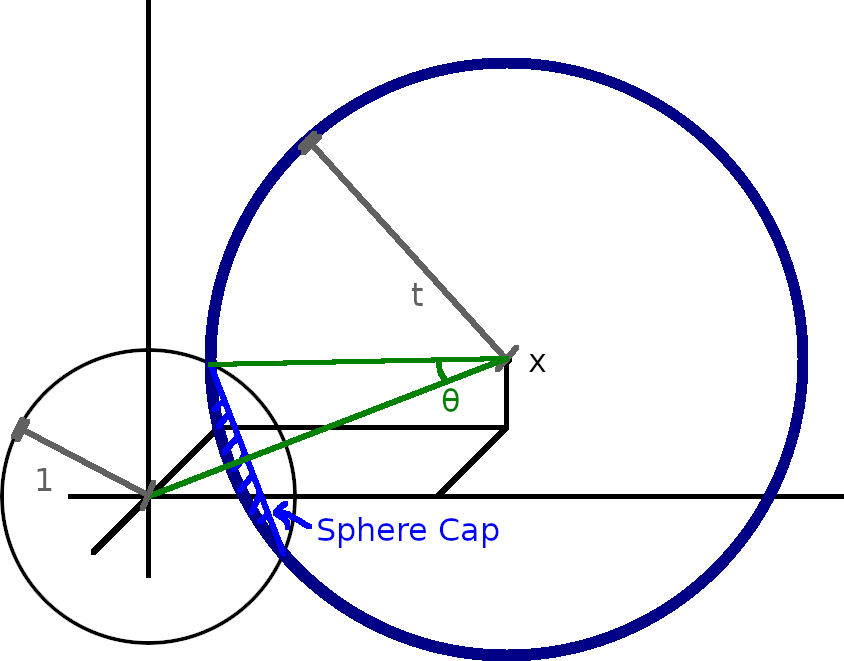
\includegraphics[width=0.5\textwidth]{spherecap.png}
  \end{center}
  \caption{Illustration of the sphere and sphere-cap the integral computes the area of}
  \label{spherecap}
\end{figure}

Then
\begin{align*}
  \tilde{U}_{tt} - \tilde{U}_{rr} = 0 & \text{ in } \reals_+ \times (0, \infty)\\
  \tilde{U} = \tilde{G}, \tilde{U}_t = \tilde{H} & \text{ on } \reals_+ \times \set{t = 0}\\
  \tilde{U} = 0 & \text{ on } \set{r = 0} \times (0, \infty)
\end{align*}

$$
u(x, t) = t \avgint_{\bndry{\ball{x}{t}}} h(y) \dd{S(y)}
$$

To compute the area of the spherical cap, we first note
$$
1 = t^2 \sin^2(\theta) + (|x| - t \cos(\theta))^2 = t^2 + |x|^2 - 2 |x| t \cos(\theta)
$$

Then, recall the surface area of a sphere cap for a sphere of radius $t$ and an angle $\theta$:
$$
A = 2 \pi t^2 (1 - \cos(\theta))
$$

Some manipulations of the previous two equations gives
$$
A = -\frac{\pi t}{|x|} \left( (|x| + t)^2 - 1 \right)
$$

Then, when $-1 < |x| - t < 1$ (since the sphere must actually intersect the unit sphere at the origin),
and $t \neq 0$, $u(x. t)$ is as follows:

$$
u(x, t) = t \frac{A}{4 \pi t^2} = -\frac{(|x| + t)^2 - 1}{4 |x|}
$$

In full:

$$
u(x, t) =
\begin{cases}
  -\frac{(|x| + t)^2 - 1}{4 |x|} & ||x| - t| < 1, t \neq 0\\
  0 & \text{otherwise}
\end{cases}
$$

To check our calculations, we can rewrite the original problem in spherical coordinates:

$$
\begin{cases}
  u_{tt} - \Delta u = u_{tt} - \frac{2}{r} u_r - u_{rr} = 0, & r > 0, \theta \in \reals^2, |\theta| = 1, t > 0\\
  u(r, \theta, 0) = 0 & r > 0, \theta \in \reals^2, |\theta| = 1\\
  u_t(r, \theta, 0) =
  \begin{cases}
    1 & r < 1\\
    0 & r > 1
  \end{cases} & r > 0, \theta \in \reals^2, |\theta| = 1
\end{cases}
$$

Our solution is

$$
u(r, \theta, t) =
\begin{cases}
  -\frac{(r + t)^2 - 1}{4 r} & |r - t| < 1, t \neq 0\\
  0 & \text{otherwise}
\end{cases}
$$

For $|r - t| < 1, t \neq 0$, we compute
\begin{align*}
  u_t = &\frac{t + r}{2 r}\\
  u_{tt} = &\frac{1}{2 r}\\
  u_r = &\frac{1 - t^2 + r^2}{4 r^2}\\
  u_{rr} = &\frac{t^2 - 1}{2 r^3}\\
  u_{tt} = &\frac{2}{r} u_r + u_{rr} = \frac{t^2 - 1}{2 r^3} - \frac{1}{2 r} + \frac{t^2 - 1}{2 r^3} = -\frac{1}{2 r}
\end{align*}

For $r < 1$, $\limitto{t}{0} u_t = \frac{1}{2}$, suggesting this is off by a factor of 2, so we amend the solution to
$$
u(r, \theta, t) =
\begin{cases}
  -\frac{(r + t)^2 - 1}{2 r} & |r - t| < 1, t \neq 0\\
  0 & \text{otherwise}
\end{cases}
$$

\end{enumerate}
\end{document}
